Una vez establecido el objetivo de este proyecto en la introducción, en este capítulo se describirán los conceptos generales necesarios para la comprensión de este documento. Para ello, en primer lugar se detalla el proceso de onboarding en proyectos software y las dificultades que presenta, junto con el trabajo previo realizado en este ámbito.

Por otro lado, se explicará a grandes rasgos qué son los agentes basados en grandes modelos de lenguaje (conocidos también por el anglicismo Large Language Models o por sus siglas LLM), su arquitectura, funcionamiento e interacción con herramientas externas. Se introduce además el Model Context Protocol como estándar de comunicación entre estos componentes.

Finalmente, se aborda el estado del arte en arquitecturas de agentes, sus aplicaciones en proyectos software y las técnicas de ajuste de modelos.

\section{Onboarding en proyectos software}
El proceso de incorporación (onboarding) de nuevos desarrolladores de software constituye un desafío persistente para las organizaciones tecnológicas, donde los recién incorporados enfrentan una sobrecarga informativa mientras los desarrolladores senior ven afectada su productividad al destinar tiempo considerable a actividades de formación y mentoría\cite{sim_ramp-up_1998}. 

Si bien prácticas como la designación de mentores han demostrado ser efectivas para facilitar la integración de nuevos miembros, estas incrementan significativamente la carga de trabajo sobre los profesionales experimentados, generando potenciales retrasos en los proyectos\cite{steinmacher_systematic_2015}.

En este contexto, los modelos de lenguaje de gran escala emergen como una alternativa prometedora para transformar el proceso de onboarding, ofreciendo orientación personalizada e instantánea que podría reducir la dependencia de los desarrolladores senior, preservar la productividad global de los equipos y facilitar una incorporación más eficiente y menos disruptiva\cite{ritz_artificial_2023}.

\subsection{Trabajo previo}

La Universidad del País Vasco, en colaboración con LKS NEXT\footnote{LKS NEXT: \url{https://www.lksnext.com/es/}}, desarrolló el prototipo denominado I Need a Hero (INAH), diseñado para aprovechar el potencial de los LLM en la localización de expertos dentro de la organización\cite{azanza_can_2024}. INAH opera en dos fases: primero crea perfiles de ``héroes'' extrayendo información de currículos de empleados dispuestos a asistir; luego, ante una consulta, utiliza GPT-3.5 para identificar las competencias requeridas y localizar a los profesionales que las poseen.

En una línea de estudio complementaria, un trabajo reciente ha presentado el sistema ``Onboarding Buddy'', el cual implementa una arquitectura multi-agente que organiza diversos componentes especializados para proporcionar asistencia contextualizada durante la incorporación de nuevos desarrolladores\cite{ionescu_multi-agent_2025}.

El sistema fundamenta su funcionamiento en la generación dinámica de planes mediante cadena de pensamiento \ref{plani}, evaluados posteriormente para determinar su posible descomposición en sub-tareas procesadas en paralelo por otros agentes.

\section{Agentes de Grandes Modelos de Lenguaje (LLM)}

Los agentes de Inteligencia Artificial son programas informáticos que implementan modelos computacionales para ejecutar diversas funciones específicas del contexto en el que se aplican. Tras siete décadas y media de investigación, los esfuerzos en el campo se han focalizado en agentes basados en grandes modelos de lenguaje. 

\subsection{Modelos LLM}

Los Grandes Modelos de Lenguaje son redes neuronales especializadas en el procesamiento del lenguaje natural que funcionan mediante un mecanismo de entrada-salida de tokens \ref{token}. Estos modelos reciben secuencias de tokens como entrada, denominada comúnmente "prompt", y generan secuencias de tokens como salida, aplicando durante este proceso las representaciones y relaciones semánticas aprendidas durante su fase de entrenamiento con extensos corpus textuales \cite{vaswani_attention_2023}.

Para comprender el funcionamiento de estos agentes, resulta imprescindible asimilar previamente conceptos como la tokenización, las representaciones vectoriales del lenguaje y el ajuste de dichos modelos.

\paragraph{Tokens}\label{token}
Los tokens constituyen la unidad mínima de texto que el modelo puede procesar. Dado que dichos modelos operan sobre estructuras matemáticas, requieren transformar el lenguaje natural en representaciones matriciales. Para lograr esta conversión, el texto se segmenta en dichas unidades mínimas, que pueden corresponder a caracteres individuales, fragmentos de texto o palabras completas. El conjunto íntegro de estas unidades reconocibles por el modelo configura su vocabulario. 

\paragraph{Representaciones vectoriales}
Constituyen vectores numéricos de dimensionalidad fija que codifican la semántica inherente a cada token. Por ejemplo, una dimensión específica podría especializarse en representar conceptos abstractos. En este contexto, la representación vectorial del token ``animal'' contendría un valor más elevado en dicha dimensión que la correspondiente al término ``gato'', reflejando su mayor grado de abstracción conceptual.

\paragraph{Ajuste de modelos instruct}
El entrenamiento \ref{anexo:entrenamiento} de los LLM se estructura en dos fases diferenciadas. La primera corresponde al preentrenamiento, donde el modelo procesa extensos conjunto de datos textuales con operaciones como intentar predecir el siguiente token en la secuencia. Esta fase permite al modelo captar las complejas estructuras sintácticas y relaciones semánticas inherentes al lenguaje natural. La segunda fase consiste en el ajuste fino, donde el modelo previamente entrenado se especializa mediante conjuntos de datos específicos y etiquetados \ref{anexo:datos_et}, optimizando su capacidad para ejecutar tareas concretas de clasificación o generación de texto.

Los agentes basados en LLM implementan en su mayoría modelos \textit{instruct}, variantes especialmente ajustadas para responder a consultas e instrucciones de usuarios. Dentro de esta categoría se encuentran GPT (base de ChatGPT\footnote{ChatGPT:\url{https://chatgpt.com}}) de OpenAI\footnote{OpenAI:\url{https://openai.com/}}, Claude Sonnet de Anthropic\footnote{Anthropic:\url{https://www.anthropic.com/}}, y LLama-Instruct de Meta\footnote{Meta: \url{https://about.meta.com/es/}}.



\subsection{Interacción con herramientas externas}
Los agentes LLM poseen la capacidad de interactuar con diversas herramientas como búsquedas web, bases de datos o interfaces de usuario. Fundamentalmente, este tipo de modelos solo genera tokens de texto, por lo que la integración de herramientas se implementa mediante palabras clave o tokens especiales que este puede incluir en su salida. Para ello, en el texto de entrada se especifica el esquema de la función a utilizar y, si decide emplearla, el modelo generará el texto correspondiente. Posteriormente, se procesa la respuesta para extraer llamadas a funciones si las hubiese.

La interacción con herramientas es típicamente alternante. Tras realizar la llamada a la herramienta, la salida de esta se utilizará como entrada para el siguiente mensaje del modelo. La figura \ref{fig:herramientas} ilustra el esquema de un agente con acceso a una API del clima. Como el modelo carece de información climática en tiempo real, se le indica en el prompt la posibilidad de invocar esta función. Al incluir la llamada en su texto de salida, se ejecuta la función y su respuesta se transmite al modelo para generar el resultado final.

\begin{figure}[H]
  \centering
  \hspace{-3.60cm}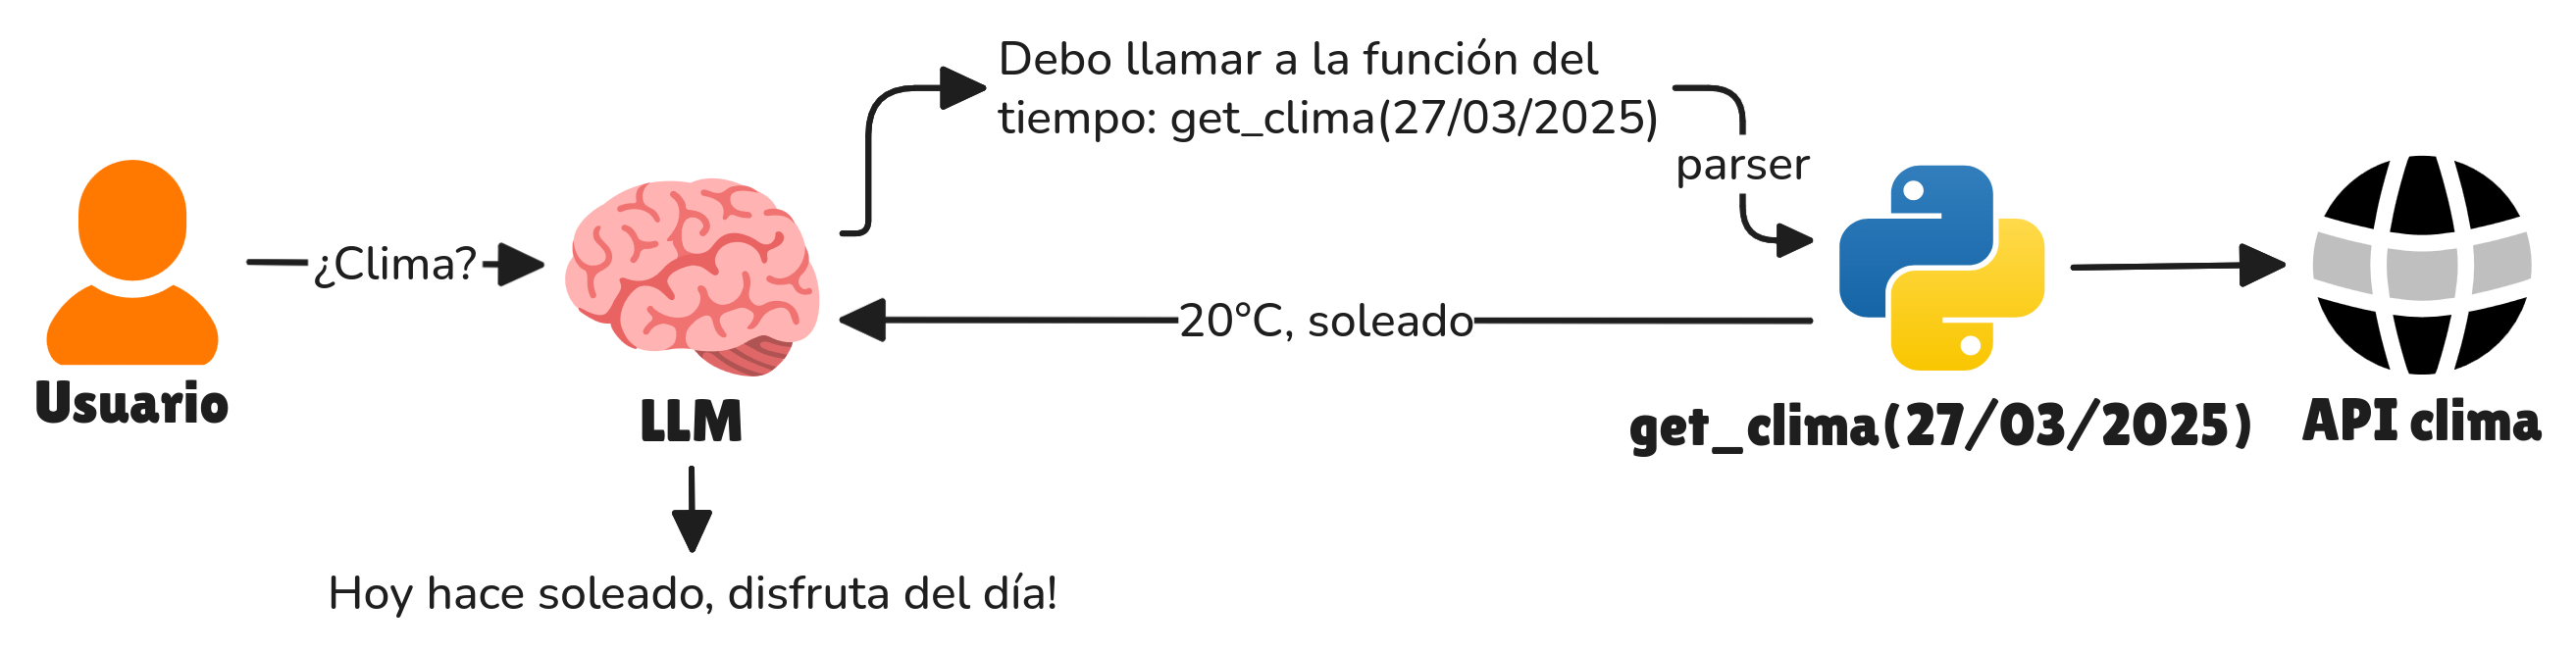
\includegraphics[width=1.25\linewidth]{figures/herramienta.png}
  \caption{Ejemplo de interacción de un modelo LLM con una herramienta externa.}
  \label{fig:herramientas}
\end{figure}


\subsubsection{Patrón ReAct}
El agente Reasoning and Act (ReAct) constituye uno de los patrones más utilizados\cite{yao_react_2023}. Se basa en un ciclo de tres pasos fundamentales: el razonamiento como generación de pensamiento sobre posibles acciones, la acción como ejecución de la herramienta seleccionada y la observación como procesamiento del resultado obtenido. Este ciclo se repite iterativamente hasta que durante la fase de razonamiento se determina que la tarea ha sido completada.

%xu_rewoo_2023 -> rewoo para no pasar observaciones a react ~orquestar
%react todo
%wang_executable_2024 -> tools con código, igual mejor donde herramientas?



\subsection{Abstracciones en frameworks}
\label{sec:abst}
En pleno auge de los agentes LLM, surgen cada vez más bibliotecas y frameworks que estandarizan su implementación. Estos marcos de trabajo ofrecen abstracciones de alto nivel para reutilizar funcionalidades comunes presentes en la mayoría de sistemas de agentes.
Las principales funcionalidades proporcionadas son las siguientes: 
\begin{itemize}
\item {\textbf{Gestión de modelos:}} La ejecución de modelos de lenguaje requiere del dominio de estos, ya que cada uno posee tokenizadores específicos \ref{anexo:tokenizer} y esquemas propios de entrada y salida. Los frameworks ofrecen interfaces unificadas, facilitando el uso de diversos modelos sin necesidad de conocimientos técnicos excesivamente detallados.
\item {\textbf{Interacción conversacional:}} La comunicación con los agentes se efectúa mediante un esquema conversacional, donde el modelo recibe un texto de entrada y genera una respuesta correspondiente. Las respuestas y entradas se concatenan secuencialmente para preservar el contexto de la conversación, cada consulta subsiguiente incorpora todos los intercambios precedentes.
\item {\textbf{Uso de herramientas externas:}} Toda la complejidad de la interacción se abstrae en el framework, por lo que el desarrollador únicamente debe especificar la función que desea incorporar.
\item {\textbf{Interacción entre agentes:}} Los agentes pueden establecer comunicación entre sí, permitiendo la construcción de sistemas con mayor complejidad. Algunos frameworks establecen protocolos que definen las modalidades de comunicación entre los distintos agentes.
\end{itemize}

Para este trabajo utilizaremos fundamentalmente LangChain\footnote{LangChain: \url{https://www.langchain.com/}} para la gestión de llamadas a APIs de modelos y prompting, LangGraph\footnote{LangGraph: \url{https://www.langchain.com/langgraph}} para la orquestación de flujos agénticos, y LangSmith\footnote{LangSmith: \url{https://www.langchain.com/langsmith}} para el seguimiento de trazas de llamadas a modelos y herramientas. Para la gestión de los conjuntos de datos y entrenamiento de modelos utilizaremos HuggingFace.\footnote{HuggingFace: \url{https://huggingface.co/}} 

\section{Model Context Protocol}
\label{sec:mcp_prots}
El Model Context Protocol (MCP), desarrollado por Anthropic, estandariza la comunicación entre agentes LLM y herramientas. Permite que aplicaciones diversas ofrezcan herramientas a agentes externos sin exponer detalles de implementación\cite{noauthor_model_nodate}.

La figura \ref{fig:mcp} ilustra el esquema operativo del protocolo. Los desarrolladores de Jira\footnote{Jira: \url{https://www.atlassian.com/es/software/jira}} y GitHub\footnote{GitHub: \url{https://github.com/}} han implementado un servidor MCP que traduce las interacciones con sus APIs y proporciona herramientas al cliente MCP. Esto permite que el desarrollador del agente se enfoque exclusivamente en conectar las herramientas del cliente con el agente, sin necesidad de interactuar con APIs externas. Asimismo, el cliente MCP gestiona la comunicación entre servidores, facilitando al agente el acceso directo a múltiples herramientas.

\begin{figure}[H]
  \centering
  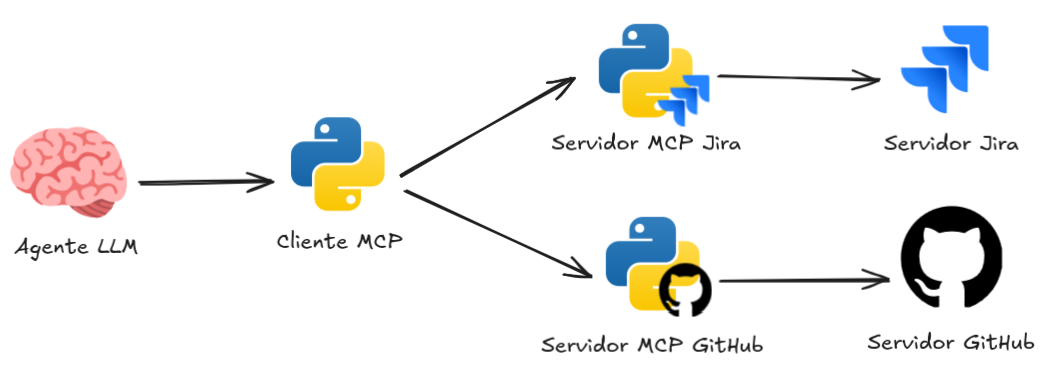
\includegraphics[width=1\linewidth]{figures/mcp.png}
  \caption{Esquema de funcionamiento del Model Context Protocol.}
  \label{fig:mcp}
\end{figure}


El protocolo ofrece dos modos de operación para establecer la comunicación entre cliente y servidor:
\begin{itemize}
  \item{\textbf{Comunicación SSE: } El protocolo Server-Sent Events (SSE) establece un canal de comunicación unidireccional sobre HTTP desde el servidor hacia el cliente. Proporciona actualizaciones en tiempo real con capacidad de streaming. En el protocolo MCP, el cliente efectúa solicitudes para la ejecución de herramientas en el servidor mediante HTTP, a lo que el servidor puede responder mediante eventos SSE.}
\item{\textbf{Comunicación STDIO: } El protocolo de entrada y salida estándar (STDIO) facilita la comunicación bidireccional entre cliente y servidor a nivel de proceso en el sistema operativo. Este mecanismo permite el intercambio de información en formato JSON a través de los canales estándar del sistema. Su diseño, orientado principalmente a entornos locales, restringe la conexión a un único cliente por servidor al limitarse a la comunicación entre dos procesos.}
\end{itemize}
La aplicación de escritorio Claude Desktop\footnote{Claude Desktop: \url{https://claude.ai/download}} de Anthropic constituye un reflejo del potencial del protocolo. Esta plataforma ofrece la posibilidad de interactuar con servidores mediante una configuración mínima. Implementando el protocolo STDIO, la aplicación ejecuta los servidores distribuidos por terceros a través de gestores de paquetes como uv\footnote{uv: \url{https://astral.sh/blog/uv}}, npx\footnote{npx: \url{https://docs.npmjs.com/cli/v8/commands/npx}} o Docker\footnote{Docker: \url{https://www.docker.com/}}. Al incorporar un cliente MCP en la aplicación, consigue integrar las herramientas disponibles en la interfaz de chat con los modelos de Anthropic.

\section{Estado del arte en arquitecturas de agentes LLM}


La comunidad científica ha diseñado diversas arquitecturas de agentes para optimizar el rendimiento de los modelos disponibles. La arquitectura RAG se distingue por complementar la entrada del modelo con información recuperada de documentos relevantes. Otras propuestas se centran en mejorar la comunicación y coordinación entre agentes.

\subsection{Arquitectura RAG}

Los modelos LLM poseen un conocimiento restringido a los datos con los que fueron entrenados. Para superar esta limitación, la arquitectura RAG (Retrieval-Augmented Generation) complementa la generación del LLM mediante la recuperación de información relevante desde repositorios de conocimiento externos. La figura \ref{fig:rag} ilustra un ejemplo de su funcionamiento.    

\begin{figure}[H]
  \centering
  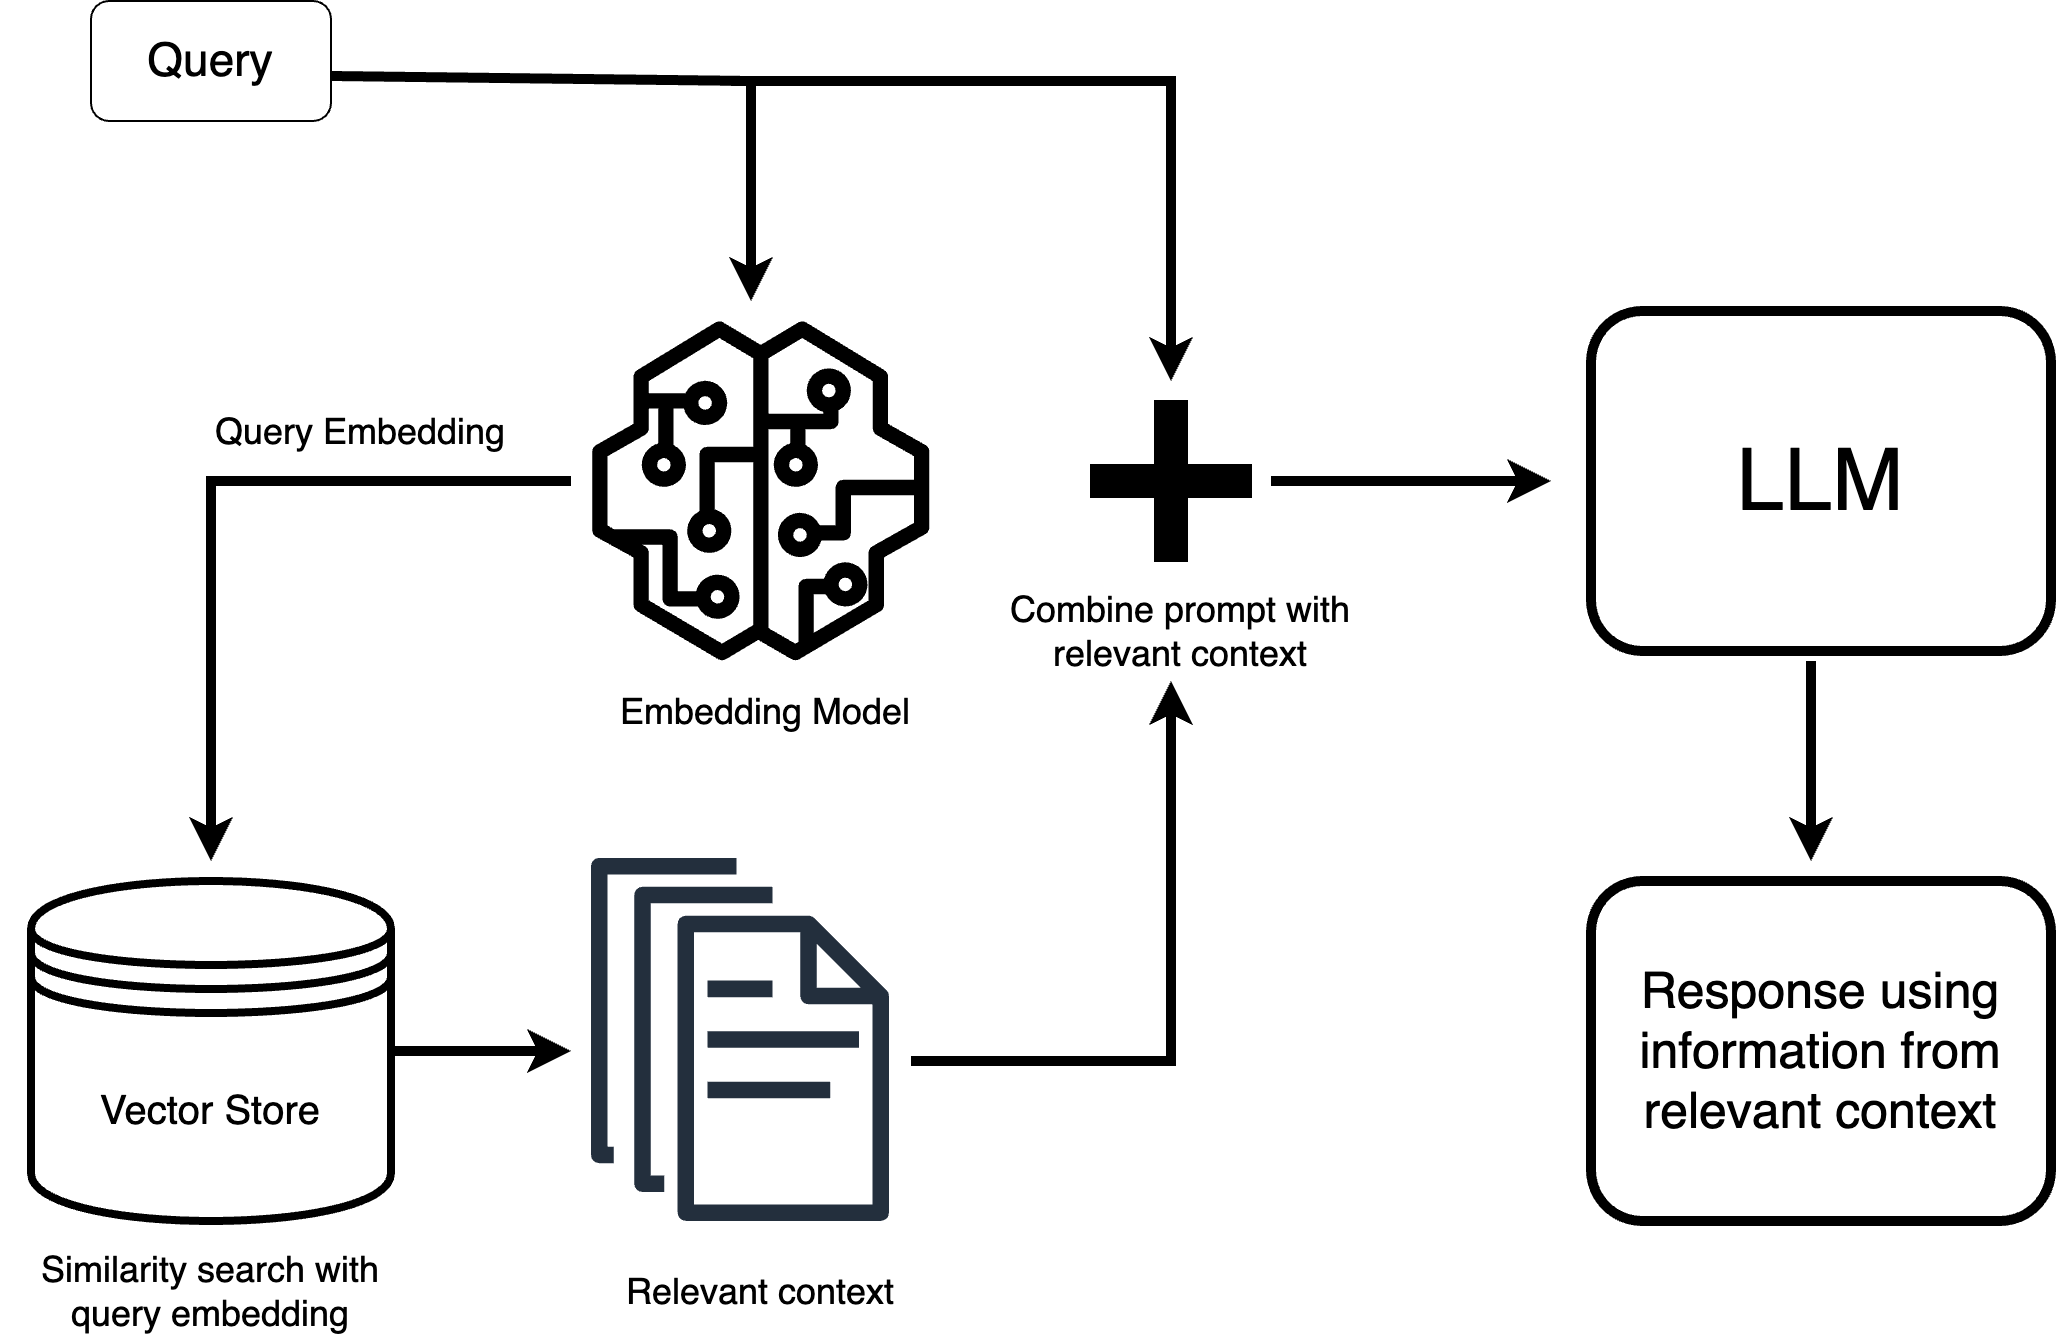
\includegraphics[width=0.75\linewidth]{figures/RAG.png}
  \caption{Esquema de funcionamiento de la arquitectura RAG en un LLM \href{https://www.clarifai.com/blog/what-is-rag-retrieval-augmented-generation}{Fuente}.}
  \label{fig:rag}
\end{figure}

La recuperación de documentos relevantes se puede implementar mediate recuperadores dispersos: expresiones regulares, búsqueda de n-gramas, palabras clave, entre otras. No obstante, el enfoque predominante consiste en el uso de recuperadores densos, conocidos como indexación vectorial. En este método, los documentos se transforman en vectores, generalmente mediante LLMs especializados en codificación, denominados Embedders. Al representar los documentos en un espacio vectorial, es posible recuperar aquellos semánticamente más pertinentes mediante la comparación del vector de consulta con los vectores de los documentos indexados, utilizando métricas como la distancia coseno \ref{anexo:dis_cos}.

\subsubsection{Estrategias RAG avanzadas}
La optimización del rendimiento en arquitecturas RAG ha sido ampliamente estudiada \cite{zhu_retrieving_2021}\cite{gao_retrieval-augmented_2024}, enfocándose en tres áreas principales: el procesado de documentos, los sistemas de recuperación y la mejora del flujo de generación.
\begin{itemize}
  \item {\textbf{Procesado de documentos:}} La calidad de la indexación documental determina la eficacia del sistema. Entre las estrategias destacadas figuran la eliminación de ruido textual, el ajuste del tamaño óptimo de los segmentos indexados, y la técnica de ventana solapada. Esta última superpone fragmentos para preservar los datos situados en las intersecciones de los segmentos. 

\item {\textbf{Sistemas de recuperación:}} Los recuperadores densos basados en representaciones, ilustrados en la figura \ref{fig:rag}, precalculan las representaciones vectoriales de los documentos mediante una indexación independiente de las consultas. Por otro lado, los recuperadores basados en interacción, proponen calcular el vector para cada documento junto al vector de consulta durante el tiempo de ejecución, obteniendo así una representación más rica que captura las relaciones contextuales específicas entre ambos elementos\cite{ma_query_nodate}\cite{levine_standing_2022}.

Para contrarrestar el sobrecoste computacional de este enfoque, se han desarrollado técnicas de indexación híbridas que combinan ambos métodos. Estas técnicas permiten realizar una búsqueda inicial utilizando representaciones vectoriales y posteriormente refinar los resultados mediante la extracción interactiva\cite{khattab_relevance-guided_2021}. 
  
\item {\textbf{Optimización del flujo de generación:}} Para tareas que requieren reflexión documentada, se han desarrollado sistemas de salto múltiple que alternan entre recuperación y generación\cite{khattab_demonstrate-search-predict_2023}\cite{shao_enhancing_2023}\cite{qi_answering_2021}\cite{zheng_take_2024}\cite{trivedi_interleaving_2023}. Estos flujos permiten al sistema examinar críticamente la información inicialmente recuperada, identificar lagunas informativas, y formular las consultas correspondientes para subsanar dichas carencias.

\end{itemize}

%lazaridou_internet-augmented_2022 -> rag con internet
%cheng_uprise_2023 -> rag sobre prompts

%li_structure-aware_2023 -> datos estructurados aprender a lenguaje natural


%kang_knowledge_2023 -> combinar RAG con GNN para relaciones 

\subsection{Arquitecturas de interacción entre agentes}
La interacción entre agentes LLM constituye un campo de investigación activo, distinguiéndose diversos avances en módulos de memoria, planificación e interacción multiagente\cite{wang_survey_2024}.
\begin{itemize}
  \item{\textbf{Módulos de memoria}}: En una interacción conversacional, el modelo procesa todos los mensajes previos, pudiendo generar un contexto excesivamente amplio. Para mitigar este problema, se han desarrollados módulos de memoria que almacenan información relevante de interacciones pasadas de forma resumida\cite{zhang_building_2024-1}\cite{fischer_reflective_2023}\cite{liang_unleashing_2023}. Esta memoria puede consultarse posteriormente mediante RAG, permitiendo recuperar los elementos más relevantes según el contexto\cite{zhao_expel_2024}.

Algunos módulos se inspiran en la estructura de la memoria humana\cite{zhong_memorybank_2024}, incorporando mecanismos que almacenan información con distintas temporalidades y niveles de relevancia\cite{wang_survey_2024}\cite{park_generative_2023}.


\item{\textbf{Planificación}}\label{plani}: Los mecanismos de planificación potencian el razonamiento de los agentes sobre sus acciones futuras.

  Entre estos mecanismos destaca el prompting de cadena de pensamiento (Chain of Thought)\cite{wei_chain--thought_2023}, que instruye al modelo para elaborar un razonamiento secuencial previo a su decisión final, permitiendo así descomponer problemas complejos paso a paso.
Partiendo de este enfoque, estrategias avanzadas como la autoconsciencia\cite{liang_unleashing_2023} lo amplían mediante la generación de múltiples cadenas de razonamiento independientes y la posterior selección de la respuesta óptima entre ellas\cite{yao_tree_nodate}\cite{wang_recmind_2024}.

De manera complementaria, las técnicas de reflexión\cite{shinn_reflexion_nodate}\cite{madaan_self-refine_nodate}\cite{miao_selfcheck_2023} implementan un proceso iterativo donde el propio modelo evalúa y refina sus respuestas.

Por otro lado, la estructuración de acciones constituye una metodología ampliamente adoptada en la planificación\cite{lin_swiftsage_nodate}\cite{huang_language_nodate}\cite{wang_describe_2024}. Esta técnica permite definir planes de alto nivel que posteriormente se desglosan en acciones específicas ejecutables por los agentes\cite{zhu_ghost_2023}\cite{song_llm-planner_2023}\cite{wang_voyager_2023}\cite{liu_odyssey_2024}. Adicionalmente, la definición de interdependencias entre estas acciones permite verificar la validez de los planes generados\cite{raman_planning_nodate}\cite{liu_llmp_2023}\cite{dagan_dynamic_2023}.

Los modelos razonadores como o1 de OpenAI o DeepSeek-R1 incorporan estas técnicas de forma nativa\cite{noauthor_deepseek-r1deepseek_r1pdf_nodate}. Estos han sido entrenados con datos que incluye ejemplos de razonamiento y planificación, lo que les permite generar respuestas que incluyen dichas estructuras.


\item{\textbf{Interacción entre agentes: }}Los sistemas multi-agente implementan una arquitectura donde diversos agentes especializados son coordinados por un componente central denominado orquestador\cite{karpas_mrkl_2022}\cite{ge_openagi_nodate}. En este paradigma, cada agente se especializa en una función particular, como la búsqueda de información, la ejecución de herramientas o la generación de texto. El orquestador evalúa las consultas entrantes y las dirige hacia el agente más competente para resolverlas.

Enfoques complementarios proponen la interacción directa entre agentes especializados como mecanismo de retroalimentación\cite{zhuge_mindstorms_2023}\cite{du_improving_nodate}. Por ejemplo, ChatDev\cite{qian_chatdev_2024} establece un sistema de colaboración entre agentes programadores, testers y gestores para abordar problemas de ingeniería de software. MetaGPT\cite{hong_metagpt_2024} refina esta propuesta al implementar un protocolo de comunicación basado en el patrón publicador/suscriptor entre los agentes, permitiéndoles difundir información de forma selectiva. 
\end{itemize}


\section{Agentes LLM en proyectos software}

La integración de agentes en proyectos software ha sido objeto de estudio enfocándose principalmente en el ámbito de la generación automática de código. Se pueden destacar tres niveles de autonomía en los productos desarrrollados: sugerencias de autocompletado, asistentes de programación y agentes autónomos. 

\begin{itemize}
  \item {\textbf{Sugerencias de autocompletado:}} GitHub Copilot\footnote{GitHub Copilot: \url{https://github.com/features/copilot}} o Cursor\footnote{Cursor: \url{https://www.cursor.com/}} ofrecen la integración de un modelo LLM ajustado para generación de código directamente al entorno del desarrollador. De esta forma, el desarrollador recibe sugerencias de autocompletado en tiempo real mientras escribe el código.  

Este tipo de herramientas han demostrado ser eficaces para aumentar la productividad de los desarrolladores en tareas de programación repetitivas\cite{kalliamvakou_research_2022}. Sin embargo, debido a su enfoque en la rapidez de respuesta, presentan limitaciones en la aplicación de razonamiento profundo.

\item {\textbf{Asistentes de programación:}} Principalmente en aplicaciones en forma de chat, herramientas como GitHub Copilot Chat, Cursor o Cody\footnote{Cody: \url{https://sourcegraph.com/cody}} de SourceGraph\footnote{SourceGraph: \url{https://sourcegraph.com/}} ofrecen un sistema de chat interactivo que permite al desarrollador realizar preguntas específicas sobre el código\cite{noauthor_github_nodate}.
  
Cabe destacar el proyecto SourceGraph, el cual al ser inicialmente de código abierto ha publicado una explicación de su funcionamiento. Proporciona un sistema avanzado de navegación de código que permite la integración del agente LLM denominado Cody.

La arquitectura de este sistema opera en dos etapas: en primera instancia, los servidores de lenguaje específicos para cada lenguaje de programación analizan la estructura del código fuente, generando un grafo de dependencias que representa las relaciones jerárquicas entre los distintos elementos del código (funciones, clases, métodos, interfaces, entre otros)\cite{noauthor_sourcegraphscip_2025}. Posteriormente, el sistema implementa un mecanismo RAG basado en trigramas sobre el grafo del proyecto, cuyos fragmentos son suministrados al agente Cody, que procesa esta información estructurada y elabora respuestas contextualizadas a las consultas del desarrollador\cite{noauthor_sourcegraphsourcegraph-public-snapshot_nodate}.

\item {\textbf{Agentes autónomos:}} Con un enfoque más ambicioso, soluciones como Aider\footnote{Aider: \url{https://aider.chat/}} o DevinAI\footnote{DeviAI: \url{https://devin.ai/}} persiguen la automatización del ciclo completo de desarrollo de software. Debido a la complejidad inherente a dicha tarea, estas herramientas permanecen en una fase incipiente\cite{acharya_devin_2025}.

  El funcionamiento de Aider presenta similitudes con SourceGraph\cite{noauthor_building_2023}. En primera instancia, analiza el código fuente mediante la biblioteca Tree-sitter\footnote{Tree-sitter: \url{https://tree-sitter.github.io/tree-sitter/}}, generando un grafo de dependencias que representa las definiciones (funciones, clases, interfaces, etc.) y las referencias entre estas. Posteriormente, implementa un algoritmo de clasificación de grafos para determinar la relevancia de cada nodo respecto al contexto actual. De este modo, incorpora dicho contexto junto con un mapa de los ficheros del proyecto en la entrada del agente LLM.  

\end{itemize}

\section{Ajuste de modelos para agentes LLM}
\subsection{Limitaciones de los modelos actuales}
Los modelos \textit{instruct} del estado del arte poseen la capacidad de resolver tareas que requieren comportamiento agéntico gracias a su amplio conocimiento general. No obstante, su eficiencia es cuestionable, puesto que para tareas específicas pueden carecer de ciertos conocimientos particulares, mientras que disponen de una cantidad considerable de información superflua. Se estima que los modelos más avanzados en la actualidad, como GPT-4o o Claude 3.7 Sonnet, contienen cientos de miles de millones de parámetros\cite{noauthor_number_2024}, lo que los convierte en prohibitivamente costosos para su ejecución en entornos locales.

Debido a estas limitaciones y por tratarse de modelos propietarios, estos están disponibles únicamente a través de API. Este modelo de acceso requiere enviar los datos a servidores externos, planteando así preocupaciones sobre la privacidad y la seguridad de la información. Esta restricción es especialmente relevante en el ámbito del desarrollo de software, donde los datos pueden incluir información sensible o confidencial.

\subsection{Enfoques de ajuste fino para agentes específicos}
Como consecuencia de estas limitación, diversos proyectos de investigación han propuesto el ajuste fino de modelos de menor dimensión para tareas agénticas específicas. Mediante esta aproximación, es posible obtener modelos con mayor precisión en las tareas requeridas, pero con una fracción del coste.

Enfoques como FireAct\cite{chen_fireact_2023} y AgentTuning\cite{zeng_agenttuning_2023} proponen el entrenamiento de dichos modelos mediante una estrategia de destilación. Esto consiste en previamente utilizar un modelo instruct de gran tamaño para generar un conjunto de datos sintéticos para las respuestas del agente. Posteriormente, se ajusta un modelo de menor tamaño utilizando este conjunto de datos, de forma que el conocimiento del modelo grande se destila en el modelo pequeño.

Adicionalmente, Agent-FLAN\cite{chen_agent-flan_2024} propone la división de dichos datos de entrenamiento en varios conjuntos de aprendizaje. Debido a que los modelos aprenden antes a interpretar el formato de entrada que a razonar sobre la acción a realizar, se propone modificar parte de las trazas de entrenamiento para que estas tengan una estructura conversacional.
De esta forma, al ajustar el modelo con las trazas originales, este aprende la estructura de entrada y llamada de herramientas, mientras que en las trazas conversacionales, el modelo aprende a razonar sobre la acción a realizar.

\subsection{Técnicas de entrenamiento eficiente}
El entrenamiento de estos modelos se realiza mediante el ajuste de los pesos de la red neuronal. Debido a que el ajuste fino del modelo completo es costoso, en contextos de bajo coste se propone el uso de la técnica de entrenamiento Low Rank Adaptation (LoRA)\cite{hu_lora_2021}. Esta técnica consiste en ajustar únicamente un subconjunto de los pesos de la red neuronal, lo que permite reducir significativamente el coste computacional del ajuste fino.




%todo en capitulo agente código:
%rana_sayplan_2023 -> robot con path de la casa -> similar a repo
%gramopadhye_generating_2023 -> mejora al anterior con few shots entorno



















